\textbf{LIME} \\

Local Interpretable Model-agnostic Explanations \\

LIME is a model allowing to explain why an algorithm made a specific decision on a specific observation. It is model-agnostic since the method can explain decisions without understanding how the classifier works. By "explaining" we mean displaying feature importance for the decision. Typical output is:

\begin{center}
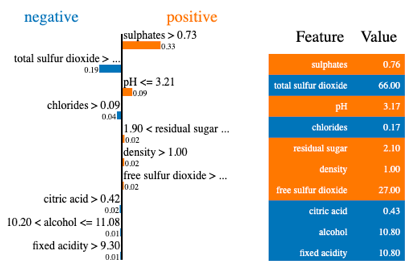
\includegraphics[scale=0.5]{LIME_wine_quality_2.png}
\end{center}

On this picture, we see the features contributing to wine quality: sulphates positively contributes to the wine quality while sulfur dioxyde contributes negatively. \\

\underline{Model} \\

The main idea behind LIME is to perturb data and learn an interpretable model locally. \\


Input: observation we want to explain $x_0$. \\

Step 1: local perturbation of $x_0$

A neighborhood is created around $x_0$. By default, LIME uses a Gaussian sampling: it generated variables from a normal distribution. Then it de-standardizes generated samples using mean and standard deviation from the observation to explain.

\textit{Note}: by default, LIME generates a neighborhood of 5000 samples. \\

Step 2: weight computation

Weights $\pi_{x_0}$ are computed according to the distance between $x_0$ and its neighbors. LIME uses an exponential smoothing kernel:
$$K(x,y) = e^{\frac{||x-y||^2_2}{\sigma^2}}$$

Reminder: $||x-y||_2 = \sqrt{\Sigma_{i=1}^n (x_i - y_i)^2}$ \\

Step 3: local classification

A linear model is used to classify samples around $x_0$. A linear model is used because it's an \textit{interpretable} model (such as decision trees).

Loss minimization to explain $x_0$:

$$\xi(x_0) = \underset{g \in G}{\operatorname{argmin}} ~\mathcal{L} (f, g, \pi_{x_0}) + \Omega(g)$$

Weights $\pi_{x_0}$ are taken into account in the loss function.

$\Omega()$ is a complexity measure. By default, LIME uses a Ridge regression, thus $\Omega()$ is the 2-norm. It would also make sense to use a lasso regularized regression (1-norm) in order to allow zero coefficients (and thus have variable selection). \\

Step 4: display explanations

Feature importance is displayed looking at regression coefficients. \\ \\